%! Author = adnansiddiquei
%! Date = 07/12/2023

\section{Solution Design}\label{sec:selection-of-solution-algorithm-and-prototyping}
    \subsection{Selection of Solution Algorithm}\label{subsec:solution-algorithm}
    Why did I choose backtracking?

    \subsection{Prototyping}\label{subsec:prototyping}
    Prior to writing any code, we prototyped the solution.
    Prototyping prior to coding allowed us to
    \begin{itemize}
        \item identify possible bugs and complexity earlier on in the development process, such that we could consider them
        prior to coding, rather than discover them after the fact;
        \item identify non-trivial and edge cases that might need to be considered while writing code and unit tests;
        \item identify API interfaces of the package, allowing us to write the unit tests beforehand (more on this when
        we talk about test driven development in Section\eqref{subsec:test-driven-development}).
        \item explore different implementations of the backtracking algorithm;
        \item identify python packages and resources that we may need to use in the implementation, and make decisions on which
        might be the most appropriate;
    \end{itemize}
    The implementation of the sudoku solver consisted of two main components: parsing the user input (and handling
    associated errors), and the backtracking algorithm itself.
    The prototyping flowcharts of these two components is shown in Fig.\eqref{fig:input-prototype} and Fig.\eqref{fig:backtracking-prototype}.
    Additionally, we wrote some \textit{pseudo-python-code} as shown in Fig.\eqref{fig:pseudocode}, allowing us to define
    the interfaces of the functions and classes that we would write - which is required to write any unit tests before prior
    to coding.
    \begin{figure}[htb]
    \centering
    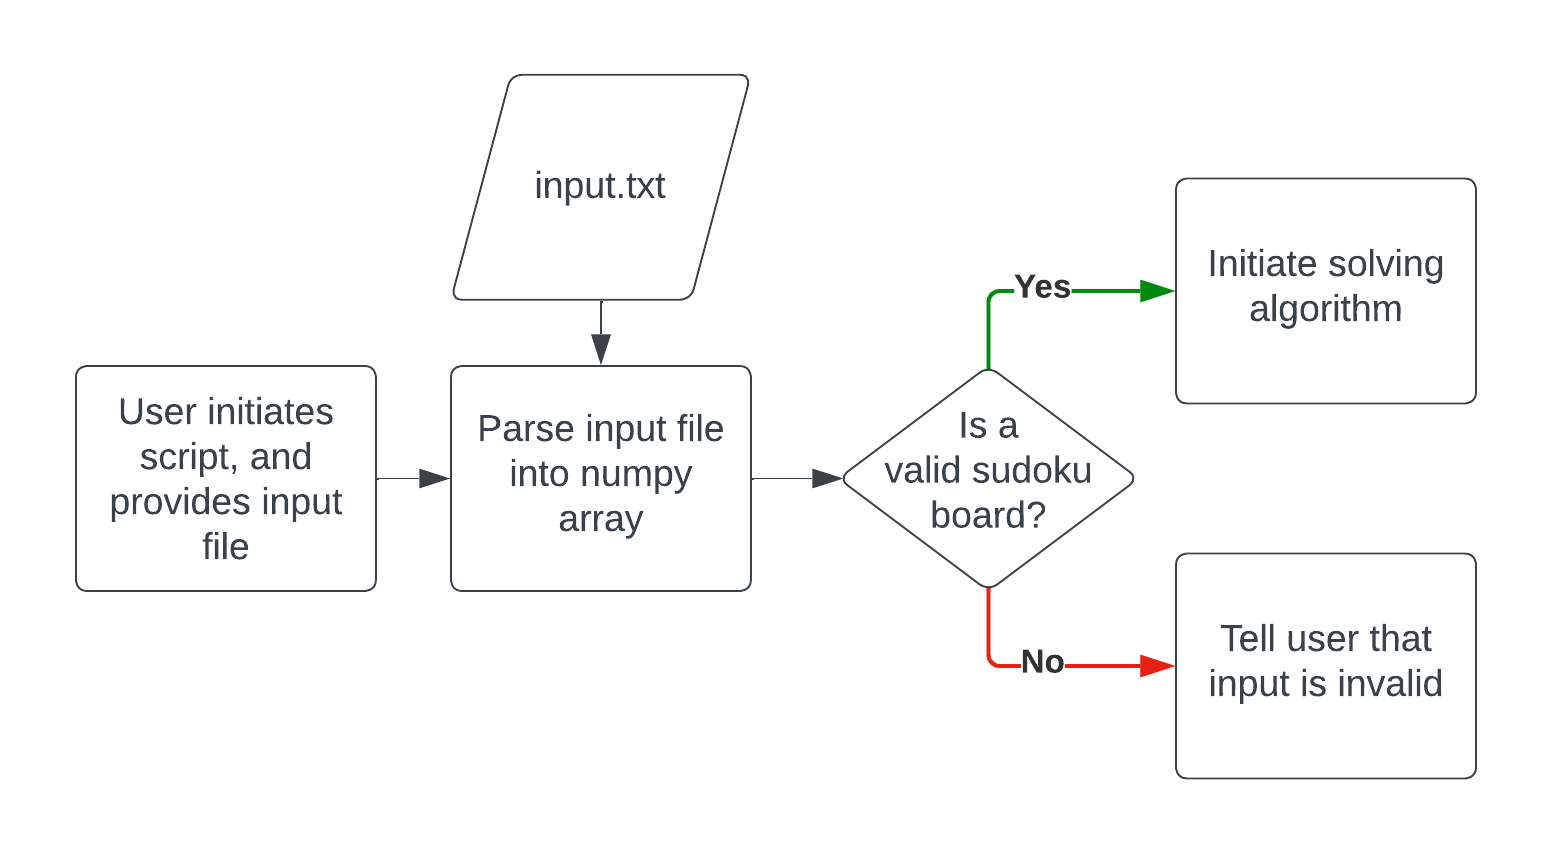
\includegraphics[width=0.9\textwidth]{./figures/parse-input-prototype}
    \caption{A flowchart for part 1 of solving a sudoku puzzle: parsing the user input.}
    \label{fig:input-prototype}
    \end{figure}

    \begin{figure}[htb]
    \centering
    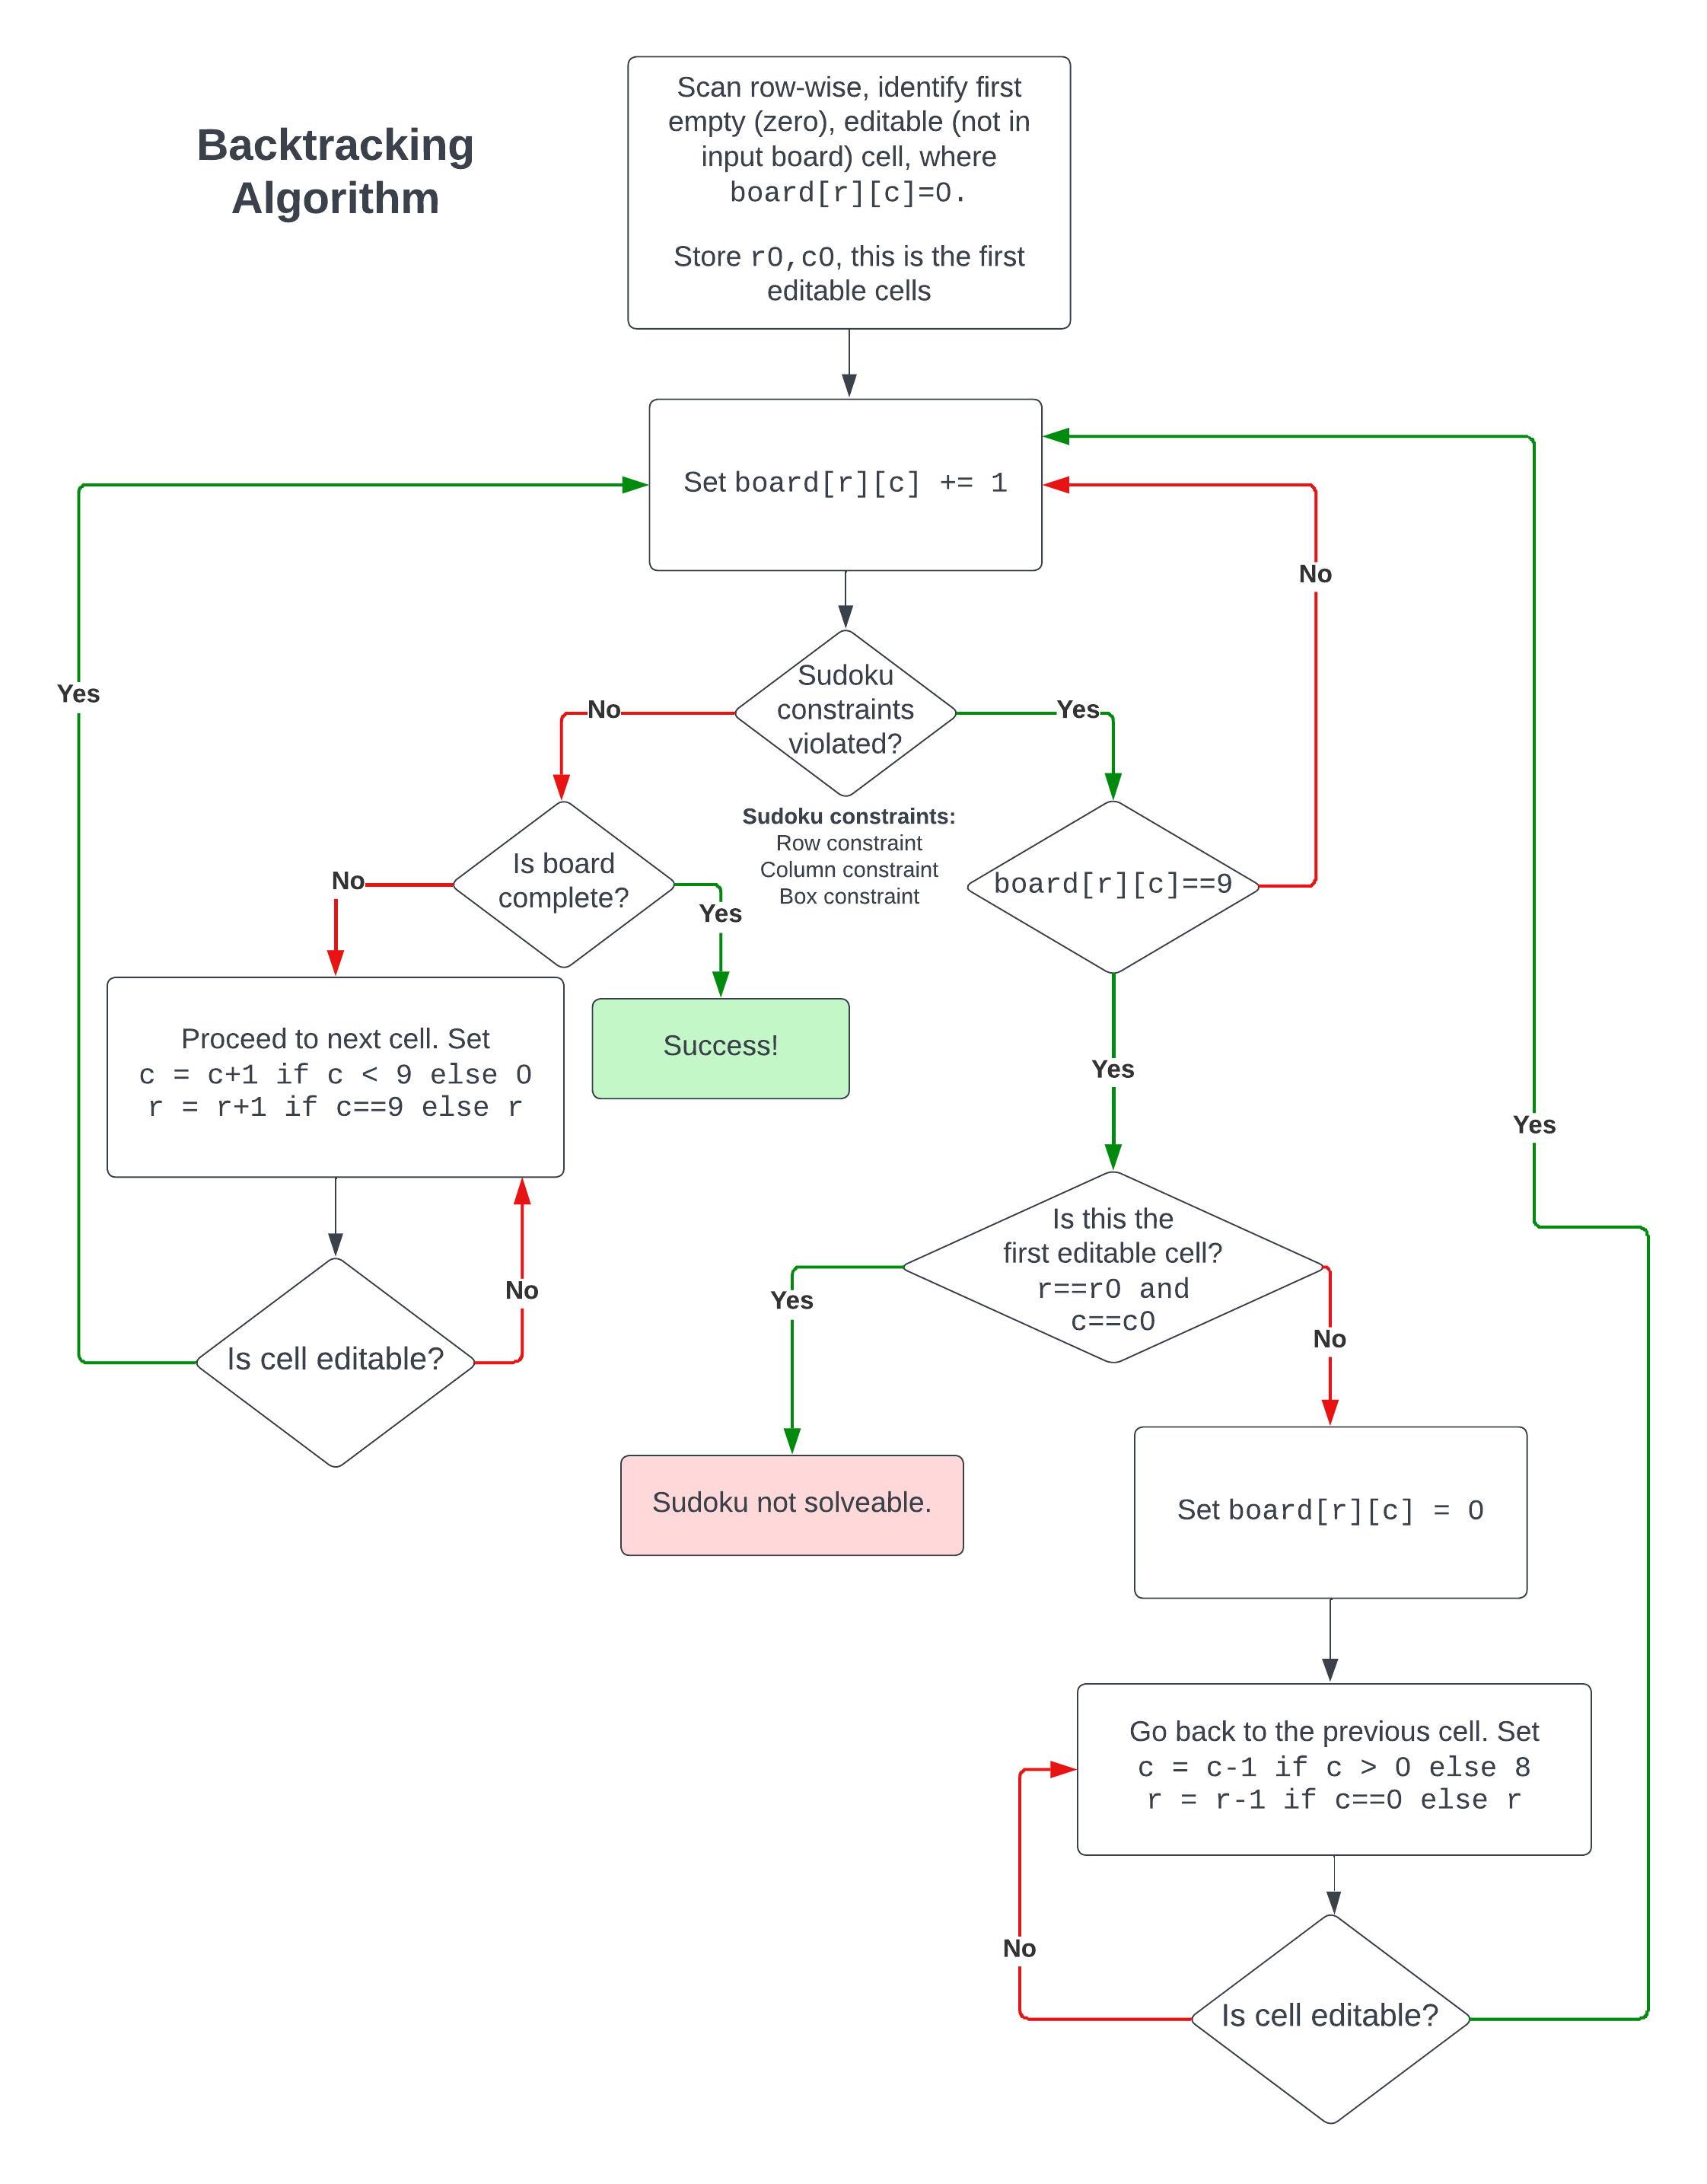
\includegraphics[width=0.9\textwidth]{./figures/backtracking-prototype}
    \caption{A flowchart for part 2 of solving a sudoku puzzle: the backtracking algorithm.}
    \label{fig:backtracking-prototype}
    \end{figure}

    \begin{figure}[htb]
    \centering
    \begin{lstlisting}[language=Python,label={lst:lstlisting}]
        class BacktrackingSolver
            def __init__(self, unsolved_board: numpy.NDArray)
                self.board  # will store solved board
                self.is_solvable  # will store whether board is solvable
                self.is_solved  # will store whether board is solved
            def solve(self) -> None:

        def parse_input_file(input_file_path: str) -> numpy.NDArray

        def save_board(
            board: numpy.NDArray,
            output_file_path: str
        ) -> None

        # entry point for script, argv = sys.argv
        def handler(argv) -> None:
    \end{lstlisting}
    \caption{\textit{pseudo-python-code} representation of the interfaces of the functions and classes within our
    \inlinecode{sudokusolver} package.}
    \label{fig:pseudocode}
    \end{figure}

    \subsection{Conclusions}\label{subsec:conclusions}
    An important decision made here was to utilise \inlinecode{numpy} arrays to represent the sudoku board, \inlinecode{numpy} is well known
    to be the most performant array manipulation package in python.
    Alternatives include using \inlinecode{pandas} or python's in-built \inlinecode{list} object, however, \inlinecode{numpy}
    is generally known to be more performant than both of these and \inlinecode{numpy} also includes numerous built-in functions
    that will likely be useful in the implementation of the backtracking algorithm.
    The tests derived from this solution design are discussed more in Section\eqref{sec:validation-unit-tests-and-ci-set-up}.
    Further iterations on these initial prototypes are discussed more in Section\eqref{sec:development-experimentation-and-profiling}
    where we discuss how experimentation and profiling changed the end implementation in efforts to optimise the code.
